\documentclass{article}
\usepackage[utf8]{inputenc}
\usepackage{amsmath}
\usepackage{amssymb}
\usepackage{graphicx}
 \usepackage{listings}


\begin{document}
\section*{Code quiz}
We are given the following code segement.
\begin{figure}[!hbt]
    \centering
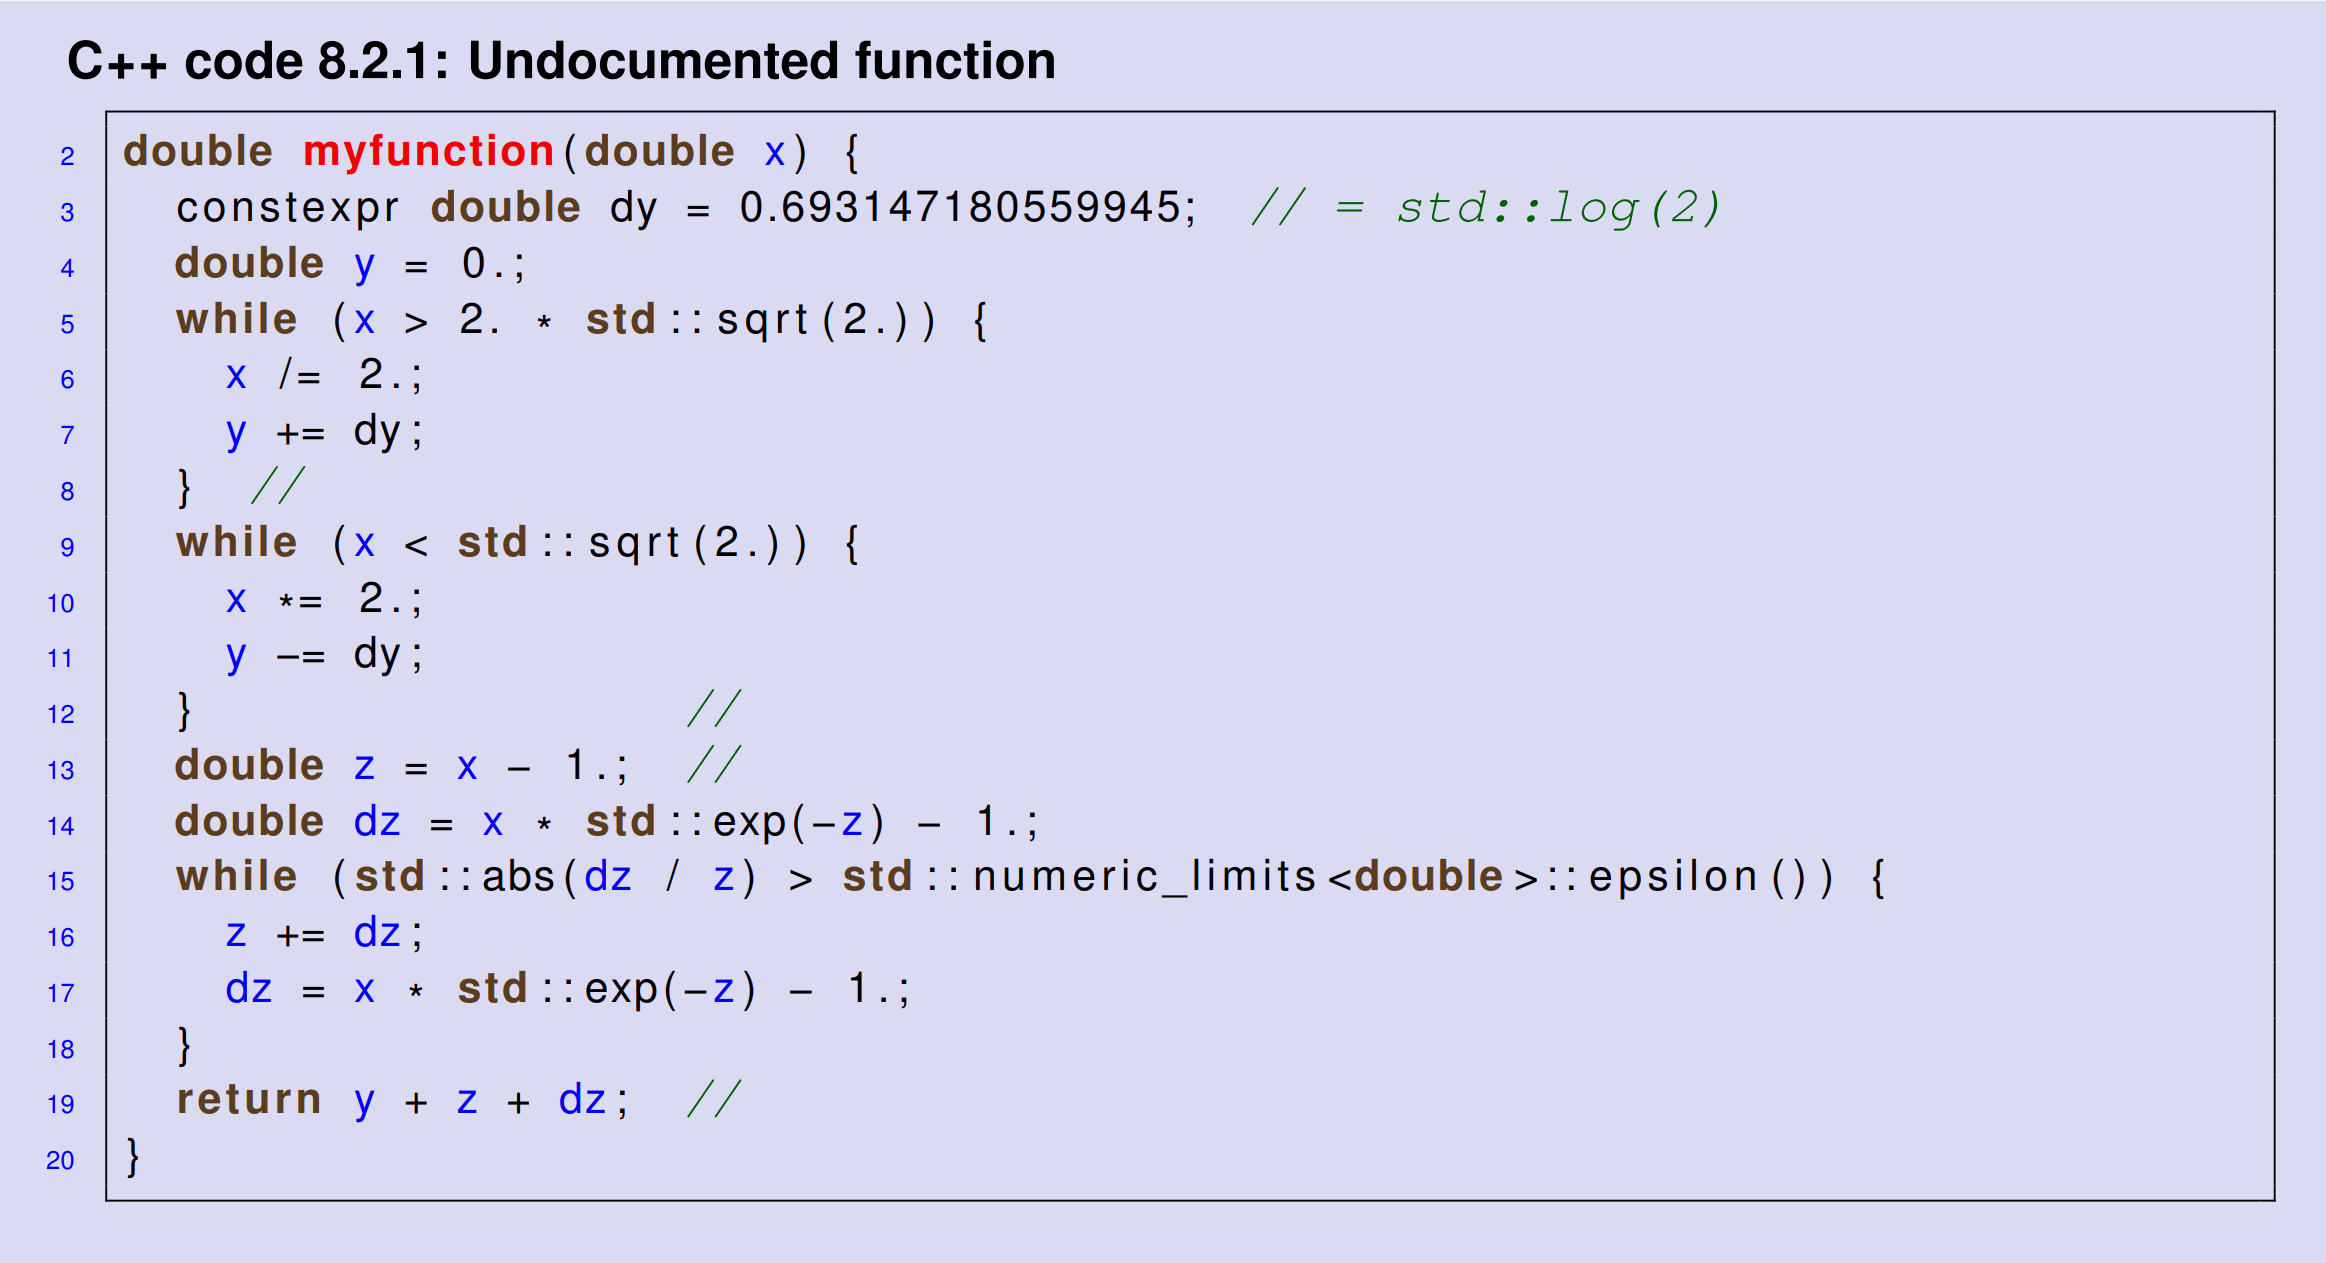
\includegraphics[width=1.0\linewidth]{UndocumentedFunction.png}
\end{figure}
\subsection*{8-2.a} 
We are tasked with finding its purpose. Seeing as the \textit{constexpr \textbf{double}} is called $\textit{dy}$ we will assume that it is a derivative. Let us have a closer look at the first while loop.

\begin{lstlisting}[language=C++,
                   directivestyle={\color{black}}
                   emph={int,char,double,float,unsigned},
                   emphstyle={\color{blue}}
                  ]
while(x > 2.0 * std::sqrt(2.0)) {
    x = x / 2;
    y = y + dy;
}
\end{lstlisting}
The \textit{\textbf{double}} variable \textit{x} is given to us as an input. We have $2 * \sqrt{2} = \sqrt{2^{2}} * \sqrt{2} = \sqrt{2^{3}} = \sqrt{8}$. Let us do an example using $x = 23.0$ we get the following loop executions, where $i$ signifies the current iteration count of the loop.
\begin{align*}
    &i = 0\: : \: x = 23.0, y = 0.0; \\
    &i = 1 \: : \: x = 11.5, y = dy \\
    &i = 2 \: : \: x = 5.75, y = 2dy \\
    &i = 3 \: : \: x = 2.875, y = 3dy \\
    &i = 4 \: : \: x = 1.4375, y = 4dy
\end{align*}
\pagebreak

\noindent Let us consider the next part of the code directly with the example.
\begin{lstlisting}[language=C++,
                   directivestyle={\color{black}}
                   emph={int,char,double,float,unsigned},
                   emphstyle={\color{blue}}
                  ]
while(x < std::sqrt(2.0)) {
    x = x * 2;
    y = y - dy;
}
\end{lstlisting}
This loop is never executed for the example above because $\sqrt{2} \leq 1.4375 < \sqrt{8}$. Can this loop ever be executed? Not if the first loop is executed. We hence see that the loop exclude each other and that only one of them can be executed. Hence we have two cases. (Assuming $x > 0$ as otherwise the code does not work properly). 
\begin{enumerate}
    \item $x > 2\sqrt{2}$ : Here we have $x = 2^{n + r}$ ($0.5 \leq r\leq 1.5$) for a positive $n$ and we hence find $y = n\log\left(2\right) = \log\left(2^{n}\right)$ and set $x$ to $x_{\text{new}}$ with $x = 2^{n} \cdot x_{\text{new}}$.
    \item $x < \sqrt{2.0}$ : Here we have $x = 2^{n+r}$ with negative $n$. We again find $y = n\log\left(2\right)$ and $x_{new}$ as described above.
\end{enumerate}
What we do here is decompose $x$ into two parts, the first part is the larger part that is a (whole number) power of $2$ and hence we can compute the logarithm easily and the second part we have to compute by approximation.


\noindent In the next part we set two variables 
\begin{lstlisting}[language=C++,
                   directivestyle={\color{black}}
                   emph={int,char,double,float,unsigned},
                   emphstyle={\color{blue}}
                  ]

\end{lstlisting}
The lines $15$ to $18$ look suspiciously like Newton iteration we have
\begin{equation*}
    \text{\textit{dz}} = \frac{x}{\text{exp}\left(z\right)} - 1 = - \left(1-\frac{x}{\text{exp}\left(z\right)}\right) = -\left(\frac{\text{exp}\left(z\right) - x}{\text{exp}\left(z\right)}\right)
\end{equation*}
So what we do in each iteration until $dz$ and $z$ are to small to be different numbers is
\begin{equation*}
    z^{\left(k+1\right)} = z^{\left(k\right)} - \left(\frac{\text{exp}\left(z\right) - x}{\text{exp}\left(z\right)}\right)
\end{equation*}
We are trying to compute $\log\left(x\right) = n \log\left(2\right) + \log\left(x_{\text{new}}\right)$ and the newton iteration computes $z \approx \log\left(x_{\text{new}}\right)$. Adding $z$ and \textit{dz} together in the last step just is one more Newton iteration. We can see that $\frac{\mathrm{d}}{dz}\left(\text{exp}\left(z\right) - x\right) = \text{exp}\left(z\right)$ we are hence determining the zero of the function
\begin{equation*}
    f\left(z\right) = e^{z} - x_{\text{new}} = 0 \implies e^{z} = x_{\text{new}} \implies \log\left(x_{\text{new}}\right) = z
\end{equation*}
which is exactly what we are looking for, which means that 
\begin{equation*}
    \text{\textit{z}} + \text{\textit{dz}} \approx \log\left(x_{\text{new}}\right)
\end{equation*}
We then return the endresult
\begin{equation*}
    \text{\textit{y}} + \text{\textit{z}} + \text{\textit{dz}} \approx n\log\left(2\right) + \log\left(x_{\text{new}}\right) = \log\left(x\right)
\end{equation*}
this is hence what the function does.

\end{document}
